%\documentclass[english, a4paper]{article}
\documentclass{llncs}
\usepackage{llncsdoc}

\usepackage{float}
\usepackage[pdftex]{graphicx}
\usepackage[font={small,it}]{caption}
\usepackage[caption=false]{subfig}
\usepackage{url}
\usepackage{siunitx}
\usepackage{graphicx}
\usepackage{pbox}
\usepackage{placeins}

\newcommand{\squeezeup}{\vspace{-8.9mm}}
\setcounter{secnumdepth}{3}
\addtolength{\textfloatsep}{-3mm}
\addtolength{\belowcaptionskip}{-15pt}



\title{Data Mining -- Assignment 2}

\author{Andrew Bedard (2566978) -- Artagan Malsagov (2562231)  -- Shabaz Sultan(2566703)}

\institute{}
\begin{document}
\maketitle
\section{Introduction}
The online travel agency (OTA) Expedia posed the challenge to rank hotels by their likelihood of being booked. In such a competitive market as the one of click-through purchases, properly ranking offered hotels according to user's preferences becomes indispensable for the OTA to win the sale. This requires an algorithm that can rank the hotels associated with a user search query. The use of ranking algorithms in the industry of online travel booking is fertile territory and the challenge provided opportunities to explore it. For further information on the competition see the Kaggle platform \cite{WinNT}.

This report details our approach to tackling this problem based on the search and click-through data provided by Expedia. First, a short review of the available literature on the topic is given. Then a description of the data and the task at hand is provided. This is followed up by a review of the methods and models used by us and how they held up to the challenge. Finally, we finish off with a summary and some concluding remarks.  

\section{Related work}
Here is a sample of the approaches of some of the groups that participated in the Expedia challenge. 

Let's start with the official winner of the competition, whose approach can be found in \cite{Zhang2013}. For the feature engineering missing values were said to be imputed by negative values, which we believe to mean the worst case is assumed. The rationale being customers don't like to book hotels with missing values. Numerical variables were bounded to remove outliers. Negative instances of booking and clicking were down-sampled. All original features were used, plus engineered features such as averages of numerical variables, price difference and categorical features converted to numerical ones. As a model an ensemble of Gradient Boosting Machines was used. 

The official runner-up also did a lot of feature engineering. Missing values were replaced by worst-case scenarios by the same reasoning as above. For instance the missing values of competitor descriptions where replaced by zero, which means data is not available. Furthermore, certain numerical features were normalized with respect to different indicators such as the prop\_id, srch\_id and month. New features were constructed such as the difference between the visitor's starrating and the starrating given to a certain property. This gave a total of 300 features on which the models LambdaMART, SVM Rank and linear regression were used. The final model used was LambdaMART. An import aspect of LambdaMART for this problem is that it can maximize non-smooth information retrieval function such as NDCG@k, which was used as an evalutation metric in this competition.

The paper \cite{DBLP:journals/corr/LiuXZYPLSW13} details an approach which meshes together several different ranking models: logistic regression, support vector machines, random forest, gradient boosting machine, factorization machine and LambdaMART, among others. The team identified the most import features as price\_usd, prop\_starrating and prop\_location\_score2. Data was balanced for training random forest, making it feasible to train with a large number of trees.  For missing values the first quartile calculated for the prop\_id of the missing data point was used. As their ensemble the team tried different linear combinations and sought the combination that would give a better result than a single model could.
 
\section{Data description}
Given a search query $x_{i}$ and the hotels $\{h_{1}^{i},\dots,h_{m_{i}}^{i}\}$ associated with it, where $\leq m_{i} \leq 38$(the maximum number of hotels associated with any search query is not more than $38$ and not less than $4$), a ranking algorithm has to estimate the scores  $\{s_{1}^{i},\dots,s_{m_{i}}^{i}\}$ corresponding to these hotel. The scores are assigned as:
$$
s_{j}^{i}=
\left\{
	\begin{array}{ll}
		5  & \mbox{if hotel $j$ was booked }   \\
		1 & \mbox{if hotel $j$ was clicked }  \\
		0 & \mbox{if hotel $j$ was neither clicked nor booked}
	\end{array}
\right.
$$
  
The data taken from Kaggle totals about $10$ million records spanned by $336,334$ search queries, meaning at least $4$ records correspond to one search query and at most $38$. The data is divided in half into a training and test set. Each record in the training data is represented by $54$-dimensional vector, where the two class variables booking and clicking and the variables for purchase amount and position in Expedia's ranked list are not included in the test set. Indeed, in our problem the target variables to be estimated are click\_bool and book\_boolean, based on which the scores for the ranking can be assigned. The remaining $50$ variables are roughly divided into search criteria, hotel characteristics (dynamic/static), history of the user and competitive OTA information. A variable not covered by these categories is whether the search result were presented in random order or based on the ranking algorithm employed by Expedia (in some cases hotels were presented in random order to learn about user preferences).

As an evaluation metric the average NDCG over all queries is used, with $k=38$ as the truncation level. Formally, $\displaystyle DCG_{k}=\sum_{i=1}^{k}\frac{2^{rel_i}-1}{\log_{2}(i+1)}$. Here $rel_{i}$ represent the true score of the hotel ranked in position $i$. Observe that only one score can be $5$: the hotel booked. The further down the summation it is placed the more it is discounted, decreasing the score. Likewise for the hotels that were clicked and it doesn't matter in which order the clicks are placed, as long as they are ranked below the booked hotel and above the hotels booked nor clicked. The ideal ranking then gives the maximal discounted gain, $IDCG_{k}$. Consequently, $NDCG_{k}=\frac{DCG_{k}}{IDCG_{k}}$ 

The data is furthermore divided into categorical and numerical variables. The categorical variables are for instance IDs for the search queries, hotels and websites of Expedia.  

Finally, there are multiple output variables, which can be represented in different ways, namely as either a score or classes for clicks and bookings. The fact is also that the NDCG is not a smooth function of the scores, which makes it hard to involve it in an online optimization process.        


\section{Working on the data}

	There were a few challenges with working on the data. First was the sheer number of records, which made direct observation and manipulation very challenging, thus from the data set approximately 10\% was selected for analysis and training. This was done by first selecting 10\% of the records, then adding further records to ensure we had complete data for each search id, that is, if we selected a record from search id \textit{x}, then all records from search id \textit{x} were added to our data.

	The second large challenge was that many of the records were incomplete. Certainly we can see in figure \ref{fig:pctM}, many of the features were missing over 80\% of their values.
	\begin{figure}[H]
	\centering
	\textbf{Percentage of missing data}\par\medskip
		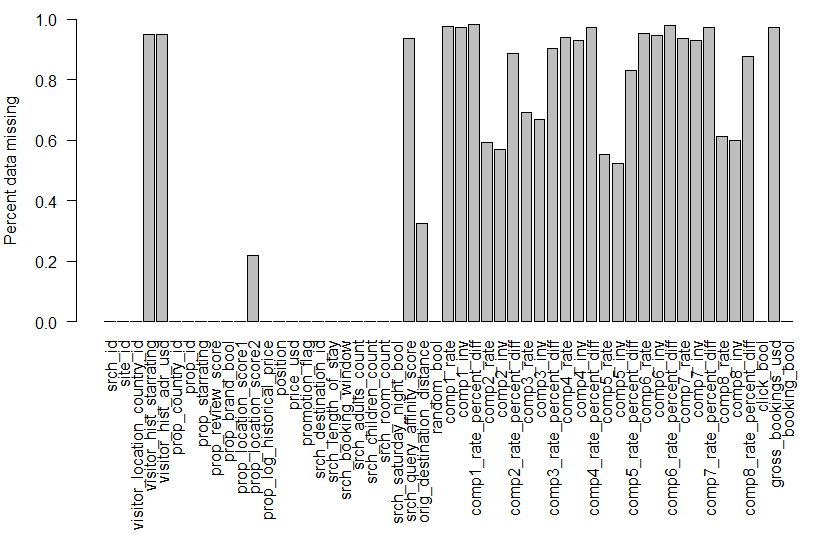
\includegraphics[scale=0.4]{figures/pct_missing.png}
	\caption{Percentage of missing data for each feature}
	\label{fig:pctM}
	\end{figure}
	
	Further, there were outliers or errors in some factors, \verb!'price_usd'! for example in our training set had a minimum of 0 and a maximum of 371493.6. It is impossible to tell exactly how this happened or what these represent, however we concluded it was due to some error and the points were treated as outliers and replaced as is stated below. 
	
	One of the salient features of the data processing procedures practised in \cite{DBLP:journals/corr/LiuXZYPLSW13} was their decision to split up features into their respective country id's, thus if they replaced the missing data for hotel star rating, they replaced it by a function of other hotels within the same country. It may make sense that people and businesses have the same behaviour within a specific country, so treating this as a reasonable assumption we also chose to replace missing factors within their country id. Simply applying experimentation we were able to arrive at a formulation for filling in missing or zero values to maximize the NDGC for our final model, they are as follow:
	\begin{itemize}
	\item \verb!'price_usd'! outliers, these were replaced with the first quantile value.
	\item missing values in \verb!'prop_location_score2'!,\verb!'visitor_hist_adr_usd!,\verb!'visitor_hist_starrating'!,\ \verb!'prop_review_score'! were replaced with their respective mean values. 
	\item Zero values in \verb!'prop_starrating'!, \verb!'prop_review_score'!, \verb!'prop_starrating'! were replaced with their respective third quantile value.
	\item Zero values in \verb!'prop_log_historical_price'! were replaced by their respective first quantile values. 
	\item Zero values of \verb!'srch_length_of_stay'! were replaced their mean values.
	\end{itemize}



\section{Models and evaluation}



\subsection{Logistic Regression}

This approach was to closely follow the procedure of \cite{DBLP:journals/corr/LiuXZYPLSW13} to create a simple Logistic Regression model, and to test the performance of the composite features outlined in their paper.

To begin, a simple Logistic Regression model was created using all of the supplied features in our 10\% training data. This was done by first creating a clicking classifier taking all features of the data into account, with a class weight set to down sample the non-clicking such that the model would not simply predict that no one ever clicks. This process was then repeated to create a booking classifier.
Finally using our two classifiers we tested on our 1\% data set, one at a time to predict booking and clicking. Using this method we achieved a NDCG score of: 0.3531, which is comparable with pure random sorting.

Several composite features were created as outlined in \cite{DBLP:journals/corr/LiuXZYPLSW13}
\[\textit{ump = exp(prop\_ log\_ historical\_ price) - price\_ usd}\]
\[\textit{price\_ diff = visitor\_ hist\_ adr\_ usd - price\_ usd}\]
\[\textit{starrating\_ diff = visitor\_ hist\_ starrating - prop\_ starrating}\]
\[\textit{per\_ fee} = \frac{\textit{price\_ usd*srch\_ room\_ count}}{\textit{srch\_ adults\_ count+srch\_ children\_ count}}\]
\[\textit{score2ma = prop\_ location\_ score2*srch\_ query\_ affinity\_ score}\]
\[\textit{total\_ fee = price\_ usd*srch\_ room\_ count}\]
\[\textit{score1d2} = \frac{\textit{prop\_ location\_ score2} + 0.0001}{\textit{prop\_ location\_ score1} + 0.0001}\]

These newly created features all fall under the top 20 relevant features as calculated by \cite{DBLP:journals/corr/LiuXZYPLSW13}, thus we fellow the procedure as above and create a new model with clicking and booking classifiers, adding in these new features. The resulting NDCG score was: 0.3535, which is a negligible gain over the previous score of 0.3531. We assumed this was due to too many features in the model, so our next test was to remove many of these features to measure any difference in performance. The features selected for inclusion were all of those included in the top 20 relevant features of Table 1 in {!!!!Liu paper!!!}, that were in the data, or were generated in the previous step. These were:\\ \verb!'prop_location_score2'!, \verb!'ump'!, \verb!'price_diff'!, \verb!'starrating_diff'!, \verb!'score1d2'!, \verb!'random_bool'!, \verb!'per_fee'!, \verb!'price_usd'!, \verb!'prop_review_score'!, \verb!'total_fee'!, \verb!'prop_starrating'!
\\
After repeating our procedure again for creating a Logistic Regression model, our NDGC score was: 0.3803, so clearly there was a increase in score. To examine the possible reason for this, consider fig:\ref{fig:corr} in which the correlations between data features for our 10\% test set are show by circle size and colour.

	\begin{figure}[H]
	\centering
	\textbf{Correlations}\par\medskip
		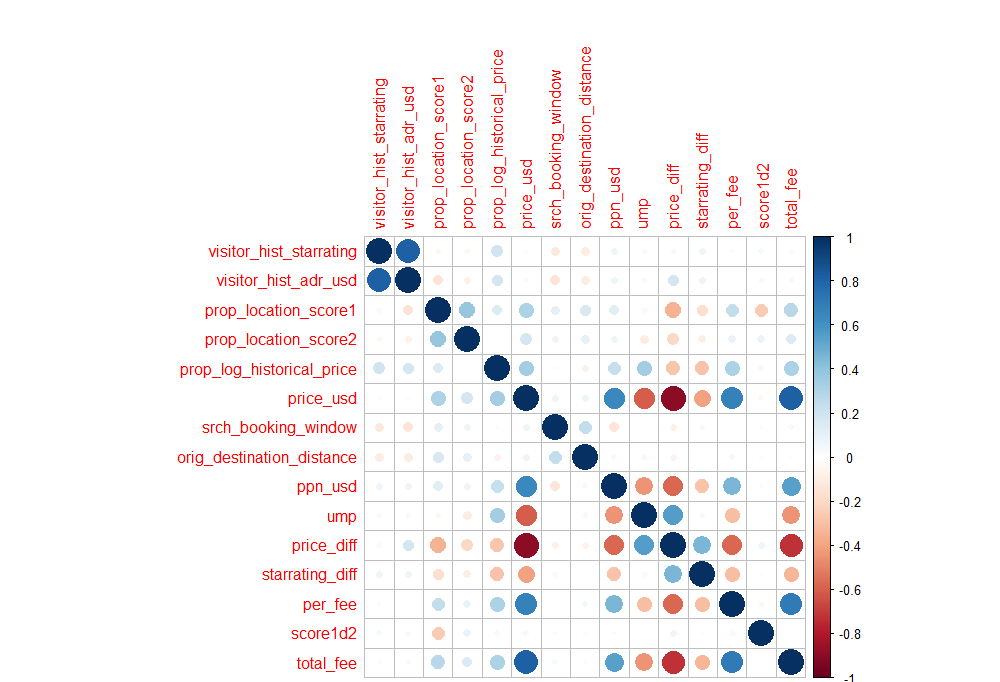
\includegraphics[scale=0.3]{figures/corr_plot.png}
	\caption{Correlations between features in model}
	\label{fig:corr}
	\end{figure}

Aside from the obvious correlations that cannot be avoided such as \textit{price\_ diff} and \textit{price\_ usd}, we can see there is a distinct lack of highly correlated features. This suggests that the features in our model thus far are likely relevant.

\subsection{Monotonic utility, feature normalization and SVM/GBM}
This approach was heavily inspired by the presentation of the official runner-up of the competition (see \cite{Wang2013}), where among other things RankSVM was used. This methods usually relies on linear separability, so the feature engineering we want to perform should reflect.

Let's start with an obviously important variable, the price of the hotels and take the log of it. This move accentuates the linearity between the price and the target variables, because log transform result in percentage changes and this way changes at higher levels of price are not wildly different from changes at lower levels of price. This is in line with the linear requirements of SVM. In this approach the $\log_{10}$ was chosen, so as to keep the engineered variable within a workable range.

A central argument in the feature engineering of the runner-up was creating variables with monotonic utility with respect to the target variables, in particular a variable that is non-increasing with respect to clicks and bookings. So as the variable increases the number of hotels clicked/booked for that variable decreases. This property comes in handy for ranking with SVM because the larger a variable for a certain hotel, the less likely that hotel is to be booked or clicked. So when training the ranking algorithm, there is a way to separate hotels that are likely to be booked from those that are not because of variables with monotonic utility.

For instance, the variable representing the star rating of the hotels does not have this monotonic utility property, as can be seen from the figure below :
 \begin{figure}[H]
     \centering
     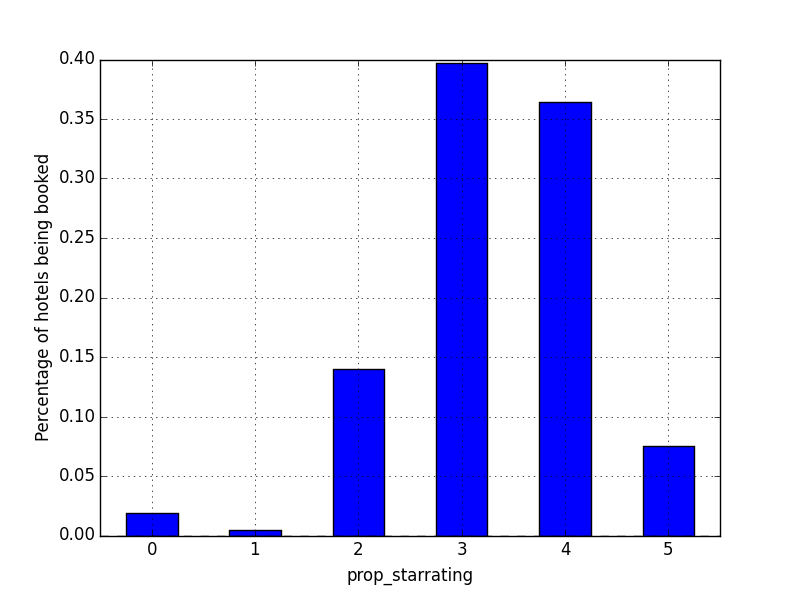
\includegraphics[width=0.60\linewidth, height=145px]{figure_normal_starrate.png}
     \caption{Fraction of booked hotels per starrating values}
     \label{fig:prop_starrating}
 \end{figure}
\noindent However, through a simple operation a new feature can be constructed with the desired property: $\textit{prop\_starrating\_monotonic} = |\textit{prop\_starrating}$ \\ 
$ - \textit{mean(prop\_starrating[booking\_bool])}|$ where the mean of the star-ratings of all booked hotels is subtracted from the regular variable \textit{prop\_starrating}, of which the absolute value is then taken. The intuition here is that the more a hotel star-rating deviates from the mean star-rating of the booked hotels, the less it is booked. Plotting a similar bar chart as the one above corroborates this intuition:
 \begin{figure}[H]
     \centering
     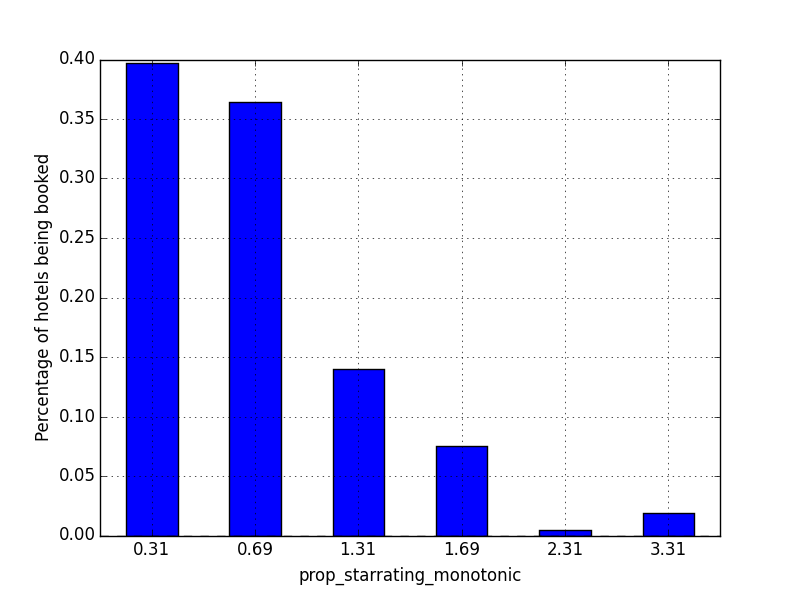
\includegraphics[width=0.60\linewidth, height=145px]{figure_monotonic_starrate.png}
     \caption{Fraction of booked hotels per feature engineered starrating values}
     \label{fig:prop_starrating}
 \end{figure}
\noindent In the plots above bookings are used as target variables, but the same can be done for clicks.

Before the log of the price was taken to make its effect on the target variables more linear. However, the prices differ per country and per time, not to mention that for some queries prices were reported on a per-day basis, while for other they were reported for the booking period indicated in the query. In order to remove these scaling factors prices will have to be normalized in an appropriate manner and the way suggested by Jun Wang, who took the second place (see \cite{Wang2013}), is to normalize prices w.r.t. certain indicators.  In this approach prices were normalized w.r.t. \textit{srch\_id}, \textit{prop\_id} and \textit{srch\_destination\_id}. Two normalization were performed: rescaling to $[0,1]$ and a standardization by the mean and standard deviation, which six extra features.

Finally, probabilities of hotels being booked or clicked were estimated. These were estimated by the fractions $\displaystyle \frac{\textit{booking(prop\_id)}}{counting(prop\_id)}$ and $\displaystyle \frac{\textit{click(prop\_id)}}{counting(prop\_id)}$ where the the number of times a hotel was booked and clicked, respectively, is divided by the number of times it appeared in the data. Naturally these probabilities cannot be estimated from the test set, but they can be estimated from the training set and then added to the test set.

As a model RankSVM was trained on the six normalized price features, the estimated probabilities for clicking and booking, the monotonic star-rating and the remaining numerical features that were not engineered. The model was slow in training and didn't perform spectacularly with a score of $0.35$. Instead, the Gradient Boosting Machines were used, which reduced training time considerably, but the score did not improve.\\
\indent The feature engineering took a long time and the reported scores were obtained from training on all features, which might have been a mistake. The six normalized prices alone were probably correlated, let alone the possibilities of unexpected correlation between the numerical features which was not checked. It would have been wise to check by trial and error which features worked best or to in a systematic way for correlations, but this was not feasible due to time constraints. 
\subsection{Commendo team approach}
The highest scoring team in the Kaggle competition was the Commendo team, part of the Opera Solutions company. They however were not granted the first place prize. We speculate that they were unwilling or unable to fully disclose their approach to Kaggle and Expedia because of use of internal tools and code that they wished to remain proprietary\footnote{A Kaggle competition admin states ``The commendo team (Michael Jahrer) achieved the highest score but was not able to fulfil all the contest requirements.'', see \url{https://www.kaggle.com/c/expedia-personalized-sort/forums/t/6203/winning-algorithm/49840#post49840}}. This made replicating their approach challenging, with only a minimal presentation to go by\cite{Jahrer2013}.\\
The approach talks about training on 19 numerical variables. We have interpreted this as being the following parameters:\\
\verb!'visitor_hist_starrating'!, \verb!'visitor_hist_adr_usd'!, \verb!'prop_starrating'!, \verb!'prop_review_score'!, \verb!'prop_brand_bool'!, \verb!'prop_location_score1'!, \verb!'prop_location_score2'!, \verb!'prop_log_historical_price'!, \verb!'price_usd'!, \verb!'promotion_flag'!, \verb!'srch_length_of_stay'!, \verb!'srch_booking_window'!, \verb!'srch_adults_count'!, \verb!'srch_children_count'!, \verb!'srch_room_count'!, \verb!'srch_saturday_night_bool'!, \verb!'srch_query_affinity_score'!, \verb!'orig_destination_distance'!, \verb!'random_bool'!. \\
The other attributes that were excluded were mostly categorical variables. The other approaches do a fair amount of feature engineering with aggregate values calculated using said categorical variables. We felt this was a good way to see how far an approach could get with more direct training on the existing numerical variables. Especially since the high score claimed to have directly trained on these and gotten very high scores using multiple different models.\\
During development instead of using the full training set a subset of 10\% was loaded. The subset was generated by a C++ program that would either select all records of a certain search id or none. This 10\% subset would then be split up again, 90\% of it in a training set and 10\% in a test set (i.e. 9\% of the original training set is trained on, 1\% to test). Again during splitting records with the same search id stick together.\\
It is not specified exactly what is trained. We implemented two binary classifiers to predict clicking and booking behaviour for each of the records in the dataset. Possibly a regression model that directly tries to predict the score would've been more accurate, but was also much slower to train so wasn't used during development. This would however be one of the first things to be looked at when doing further development on this model.\\
It is also not specified exactly how empty positions in the dataset are filled in. We opted to just use the mean of an attribute to fill in empty positions.\\
When training the classifiers using a stochastic gradient descent (SGD) learned linear classifier we get a score of \textbf{0.349}. When using a gradient boosting classifiers we also get a score of \textbf{0.349}. These are score comparable with pure random sorting. \\
One thing we noticed during exploration is that the dataset is very much biased towards negative instances, i.e. records where no clicking or booking occurs. When training classifiers this means that they very much want to just always predict the negative case, because this results in pretty high accuracy. To mitigate this we undersample the negative instance. When training the classifier that predicts the booking boolean we select all records with a booking and then select a subset of the non-booking records that is equal in size to the set of booking records. We do the same with clicking classifier.\\
Now with the trainingsets with undersampled negative instances we still get a score of \textbf{0.345} for the SGD classifiers. The gradient boosting classifiers however get a score of \textbf{0.392}. This is not terribly high, but is at least discernibly higher than a random score.\\
The Commendo team also talks about adding aggregate values to the dataset, where we group on the \verb!prop_id! and  calculate mean, median and standard deviation for each of the numerical attributes they train on. When we add all these aggregate attributes the number of attributes are so high that the system cannot train on it and always give a score equivalent to random.\\
Instead we added aggregate variables based on only one of the numerical attributes at a time. This also results in scores that don't go above 0.36. We have tried training with undersampling and not undersampling negative instances.
\section{Final Model and Results}
For the final approach we ended up combining the training and evaluation code developed for the Commendo team approach with the feature engineering and attribute selection code from the approach based on \cite{DBLP:journals/corr/LiuXZYPLSW13}. With undersampling of negative instances and training two binary gradient boosted classifiers on a 10\% subset with 9\% for training and 1\% for testing we get a score of \textbf{0.409}. This was the model we used to generate our final prediction. While we did not do proper x-fold cross validation, during development we did regenerate the subsets a few times to get a more accurate sense of the score, with the range of scores being roughly 0.40-0.45.\\
Learning the same model with SGD classifiers gets a score of \textbf{0.369} on the same training and test sets. \\
We can explore this model a bit beyond the point it was at when we submitted our prediction. If we remove undersampling of negative instances we get a score of \textbf{0.349} using the boosted gradient classifiers and \textbf{0.359} using the SGD classifiers. Clearly the undersampling improves accuracy. It also makes the training time a lot quicker, especially when training on the full trainingset.\\
We can also try adding one of the original numerical attributes to the subset we used to generate our final solution, plus aggregate attributes (mean, median, standard deviation) based on \verb!prop_id! grouping to see what this does to the score. Again using gradient boosting model and the same training and test subset we get in all cases scores less than 0.37.\\
If we add single numerical attributes without aggregate variables we're actually able to get close to the score without adding anything, but not outperform it by any significant margin. We look at another trainingset with negative instance being undersampled that has a baseline score of \textbf{0.448} (the score partially vary because of the random nature of undersampling). Adding \verb!prop_log_historical_price!, \verb!srch_saturday_night_bool! or \verb!prop_starrating! gives scores of respectively \textbf{0.442}, \textbf{0.442} and \textbf{0.447}.\\
Even taking some variability into account from generating out training subset and undersampling methods, this makes it seem likely that the most na\"ive additions of extra attributes our aggregate values will not likely improve score by a noticeable margin.

\section{Discussion}
All our models were based on binary classifiers that predicted clicking or booking and only indirectly predicted the score we're sorting on. This was done because of the speed it can be trained at. Training a regression model that directly predicts the score takes a lot longer, but is conceptually not a lot more complicated. Based on some preliminary testing our code would need minimal adaptation to try this out. This would be an obvious thing to try when we want to further research our developed models.\\
We have done selection of subsets of the attributes based on data exploration and literature. It would be interesting to look at more systematic approaches of building up minimal subset of attributes that maximize score. Looking at formal dimensional reduction methods may also be useful.\\
A lot of the most successful approaches were ensemble methods. This motivated the development of multiple independent models, with the goal of blending them together. We however didn't end up with different models that were all equally viable. It would be very interesting to see if with more time we could get all three approaches to be viable by themselves (which we will define very informally as having a score over 0.4) and then blending them to see if that gives a higher score than any of the input models.
\section{Conclusions}
We have looked at a dataset of significant size and have been able to successfully explore it and use it for predictions. These predictions compare unfavourably with the top scorers in the Kaggle competition, but is at least noticeably different from pure random predictions. By choosing to structure our approach around explicitly replicating multiple existing approaches we were able to make review of parts the literature specific to this competition. We were not able to compare them in terms of score, but also in terms of replicability, which is one of the cornerstones of the modern scientific method.\\
While we did not do any formal blending as seen with ensemble methods, by developing multiple models and making the choice of doing this in Python code, we were able successfully able to pull parts of one model (e.g. attribute selecting and feature generation) and combine it with parts of other models (e.g. data subsampling and training code) and have that combined model outperform the models that provided its parts.
\bibliographystyle{plain}
\bibliography{report}
\end{document}
